\section{IDD Conventions}\label{idd-conventions}

The following is a basic description of the structure of the IDD (it's actually taken directly from the IDD file). As noted within, \textbf{!} signifies a comment character as does the \textbf{\textbackslash{}}. \textbf{\textbackslash{}} has also been adopted as a convention for including more specific comments about each field in an object. These have been used with success in the IDFEditor and it is hoped the flexibility will provide other interface developers with useful information.

\begin{lstlisting}
!IDD_Version VERSION NUMBER
! **************************************************************************
! This file is the Input Data Dictionary (IDD) for EnergyPlus.
! The IDD defines the syntax and data model for each type of input "Object."
! Lines in EnergyPlus input files (and IDD) are limited to 500 characters.
!
! Object Description
! ------------------
! To define an object (a record with data), develop a key word that is unique
! Each data item to the object can be A (Alphanumeric string) or N (numeric)
! Number each A and N.  This will show how the data items will be put into the
! arrays that are passed to the Input Processor "Get" (GetObjectItem) routines.
! All alpha fields are limited to 100 characters.  Numeric fields should be
! valid numerics (can include such as 1.0E+05) and are placed into double
! precision variables.
!
! NOTE: Even though a field may be optional, a comma representing that field
!   must be included (unless it is the last field in the object).  Since the
!   entire input is "field-oriented" and not "keyword-oriented", the EnergyPlus
!   Input Processor must have some representation (even if blank) for each
!   field.
!
! Object Documentation
! --------------------
! In addition, the following special comments appear one per line and
! most are followed by a value.  Comments may apply to a field or the object
! or a group of objects.
!
! Field-level comments:
!
!  \field           Name of field
!                     (should be succinct and readable, blanks are encouraged)
!
!  \note            Note describing the field and its valid values. If multiple lines,
!                   start each line with \note. Limit line length to 100 characters.
!
!  \required-field  To flag fields which may not be left blank
!                     (this comment has no "value")
!
!  \begin-extensible  Marks the first field at which the object accepts an extensible
!                   field set.  A fixed number of fields from this marker define the
!                   extensible field set, see the object code \extensible for
!                   more information.
!
!  \units           Units (must be from EnergyPlus standard units list)
!                   EnergyPlus units are standard SI units
!
!  \ip-units        IP-Units (for use by input processors with IP units)
!                   This is only used if the default conversion is not
!                   appropriate.
!
!  \unitsBasedOnField  For fields that may have multiple possible units, indicates
!                   the field in the object that can be used to determine
!                   the units. The field reference is in the A2 form.
!
!  \minimum         Minimum that includes the following value
!
!  \minimum>        Minimum that must be > than the following value
!
!  \maximum         Maximum that includes the following value
!
!  \maximum<        Maximum that must be < than the following value
!
!  \default         Default for the field (if N/A then omit entire line)
!
!  \deprecated      This field is not really used and will be deleted from the object.
!                   The required information is gotten internally or
!                   not needed by the program.
!
!  \autosizable     Flag to indicate that this field can be used with the Auto
!                   Sizing routines to produce calculated results for the
!                   field.  If a value follows this, then that will be used
!                   when the "Autosize" feature is flagged.  To trigger
!                   autosizing for a field, enter Autosize as the field's
!                   value.  Only applicable to numeric fields.
!
!  \autocalculatable Flag to indicate that this field can be automatically
!                   calculated. To trigger auto calculation for a field, enter
!                   Autocalculate as the field's value.  Only applicable to
!                   numeric fields.
!
!  \type            Type of data for the field -
!                     integer
!                     real
!                     alpha       (arbitrary string),
!                     choice      (alpha with specific list of choices, see
!                                 \key)
!                     object-list (link to a list of objects defined elsewhere,
!                                  see \object-list and \reference)
!                     external-list (uses a special list from an external source,
!                                    see \external-list)
!                     node        (name used in connecting HVAC components)
!
!  \retaincase      Retains the alphabetic case for alpha type fields
!
!  \key             Possible value for "\type choice" (blanks are significant)
!                     use multiple \key lines to indicate all valid choices
!
!  \object-list     Name of a list of user-provided object names that are valid
!                     entries for this field (used with "\reference")
!                     see Zone and BuildingSurface:Detailed objects below for
!                     examples.
!                  ** Note that a field may have multiple \object-list commands.
!
!  \external-list   The values for this field should be selected from a special
!                   list generated outside of the IDD file. The choices for the
!                   special lists are:
!                        autoRDDvariable
!                        autoRDDmeter
!                        autoRDDvariableMeter
!                   When one of these are selected the options for the field
!                   are taken from the RDD or MDD file or both.
!
!  \reference       Name of a list of names to which this object belongs
!                     used with "\type object-list" and with "\object-list"
!                     see Zone and BuildingSurface:Detailed objects below for
!                     examples:
!
!                        Zone,
!                          A1 , \field Name
!                               \type alpha
!                               \reference ZoneNames
!
!                        BuildingSurface:Detailed,
!                          A4 , \field Zone Name
!                               \note Zone the surface is a part of
!                               \type object-list
!                               \object-list ZoneNames
!
!             For each zone, the field "Name" may be referenced
!             by other objects, such as BuildingSurface:Detailed, so it is
!             commented with "\reference ZoneNames"
!             Fields that reference a zone name, such as BuildingSurface:Detailed's
!             "Zone Name", are commented as
!             "\type object-list" and "\object-list ZoneNames"
!             ** Note that a field may have multiple \reference commands.
!             ** This is useful if the object belongs to a small specific
!             object-list as well as a larger more general object-list.
!
! Object-level comments:
!
!  \memo            Memo describing the object. If multiple lines, start each line
!                   with \memo.
!                   Limit line length to 100 characters.
!
!  \unique-object   To flag objects which should appear only once in an idf
!                     (this comment has no "value")
!
!  \required-object To flag objects which are required in every idf
!                     (this comment has no "value")
!
!  \min-fields      Minimum number of fields that should be included in the
!                   object.  If appropriate, the Input Processor will fill
!                   any missing fields with defaults (for numeric fields).
!                   It will also supply that number of fields to the "get"
!                   routines using blanks for alpha fields (note -- blanks
!                   may not be allowable for some alpha fields).
!
!  \obsolete        This object has been replaced though is kept (and is read)
!                   in the current version.  Please refer to documentation as
!                   to the dispersal of the object.  If this object is
!                   encountered in an IDF, the InputProcessor will post an
!                   appropriate message to the error file.
!                   usage:  \obsolete New = >[New object name]
!
!  \extensible:<\#>  This object is dynamically extensible -- meaning, if you
!           change the IDD appropriately (if the object has a simple list
!           structure -- just add items to the list arguments (i.e. BRANCH
!           LIST). These will be automatically redimensioned and used during
!           the simulation. <\#> should be entered by the developer to signify
!           how many of the last fields are needed to be extended (and EnergyPlus
!           will attempt to auto-extend the object).  The first field of the first
!           instance of the extensible field set is marked with \begin-extensible.
!
!  \begin-extensible See previous item, marks beginning of extensible fields in
!                   an object.
!
!  \format          The object should have a special format when saved in
!                   the IDF Editor with the special format option enabled.
!                   The options include SingleLine, Vertices, CompactSchedule,
!                   FluidProperties, ViewFactors, and Spectral.
!                   The SingleLine option puts all the fields for the object
!                   on a single line. The Vertices option is used in objects
!                   that use X, Y and Z fields to format those three fields
!                   on a single line.
!                   The CompactSchedule formats that specific object.
!                   The FluidProperty option formats long lists of fluid
!                   properties to ten values per line.
!                   The ViewFactor option formats three fields related to
!                   view factors per line.
!                   The Spectral option formats the four fields related to
!                   window glass spectral data per line.
!
!   \reference-class-name Adds the name of the class to the reference list
!                   similar to \reference.
!
! Group-level comments:
!
!  \group          Name for a group of related objects
!
!
! Notes on comments
! -----------------
!
! 1.  If a particular comment is not applicable (such as units, or default)
! then simply omit the comment rather than indicating N/A.
!
! 2.  Memos and notes should be brief (recommend 5 lines or less per block).
! More extensive explanations are expected to be in the user documentation
\end{lstlisting}

\subsection{IDD -- IP Units}\label{idd-ip-units}

In addition, the IDD contains indications of IP (inch-pound) units for the EnergyPlus standard SI (Systems International) units. These may be used by input and output interfaces to display values in the IP system. As noted, if the IP units are ``standard'' (first block below), then no \textbackslash{}ip-units is expected in the field. Note that for some fields -- due to their multiple use (for example, schedule values) -- there cannot be a ip-unit designation.

\begin{lstlisting}

! Default IP conversions (no \ip-units necessary)
  !      $/(m3/s)               = >   $/(ft3/min)         0.000472000059660808
  !      $/(W/K)                = >   $/(Btu/h-F)         0.52667614683731
  !      $/kW                   = >   $/(kBtuh/h)         0.293083235638921
  !      $/m2                   = >   $/ft2               0.0928939733269818
  !      $/m3                   = >   $/ft3               0.0283127014102352
  !      (kg/s)/W               = >   (lbm/sec)/(Btu/hr)  0.646078115385742
  !      1/K                    = >   1/F                 0.555555555555556
  !      1/m                    = >   1/ft                0.3048
  !      A/K                     = >   A/F                 0.555555555555556
  !      C                      = >   F                   1.8 (plus 32)
  !      cm                     = >   in                  0.3937
  !      cm2                    = >   inch2               0.15500031000062
  !      deltaC                 = >   deltaF              1.8
  !      deltaJ/kg              = >   deltaBtu/lb         0.0004299
  !      g/GJ                   = >   lb/MWh              0.00793664091373665
  !      g/kg                   = >   grains/lb           7
  !      g/MJ                   = >   lb/MWh              7.93664091373665
  !      g/mol                  = >   lb/mol              0.0022046
  !      g/m-s                  = >   lb/ft-s             0.000671968949659
  !      g/m-s-K                = >   lb/ft-s-F           0.000373574867724868
  !      GJ                     = >   ton-hrs             78.9889415481832
  !      J                      = >   Wh                  0.000277777777777778
  !      J/K                    = >   Btu/F               526.565
  !      J/kg                   = >   Btu/lb              0.00042986
  !      J/kg-K                 = >   Btu/lb-F            0.000239005736137667
  !      J/kg-K2                = >   Btu/lb-F2           0.000132889924714692
  !      J/kg-K3                = >   Btu/lb-F3           7.38277359526066E-05
  !      J/m2-K                 = >   Btu/ft2-F           4.89224766847393E-05
  !      J/m3                   = >   Btu/ft3             2.68096514745308E-05
  !      J/m3-K                 = >   Btu/ft3-F           1.49237004739337E-05
  !      K                      = >   R                   1.8
  !      K/m                    = >   F/ft                0.54861322767449
  !      kg                     = >   lb                  2.2046
  !      kg/J                   = >   lb/Btu              2325.83774250441
  !      kg/kg-K                = >   lb/lb-F             0.555555555555556
  !      kg/m                   = >   lb/ft               0.67196893069637
  !      kg/m2                  = >   lb/ft2              0.204794053596664
  !      kg/m3                   = >   lb/ft3              0.062428
  !      kg/m-s                 = >   lb/ft-s             0.67196893069637
  !      kg/m-s-K               = >   lb/ft-s-F           0.373316072609094
  !      kg/m-s-K2              = >   lb/ft-s-F2          0.207397818116164
  !      kg/Pa-s-m2             = >   lb/psi-s-ft2        1412.00523459398
  !      kg/s                   = >   lb/s                2.20462247603796
  !      kg/s2                  = >   lb/s2               2.2046
  !      kg/s-m                 = >   lb/s-ft             0.67196893069637
  !      kJ/kg                  = >   Btu/lb              0.429925
  !      kPa                    = >   psi                 0.145038
  !      L/day                  = >   pint/day            2.11337629827348
  !      L/GJ                   = >   gal/kWh             0.000951022349025202
  !      L/kWh                  = >   pint/kWh            2.11337629827348
  !      L/MJ                   = >   gal/kWh             0.951022349025202
  !      lux                    = >   foot-candles        0.092902267
  !      m                      = >   ft                  3.28083989501312
  !      m/hr                   = >   ft/hr               3.28083989501312
  !      m/s                    = >   ft/min              196.850393700787
  !      m/s                    = >   miles/hr            2.2369362920544
  !      m/yr                   = >   inch/yr             39.3700787401575
  !      m2                     = >   ft2                 10.7639104167097
  !      m2/m                   = >   ft2/ft              3.28083989501312
  !      m2/person              = >   ft2/person          10.764961
  !      m2/s                   = >   ft2/s               10.7639104167097
  !      m2-K/W                 = >   ft2-F-hr/Btu        5.678263
  !      m3                     = >   ft3                 35.3146667214886
  !      m3                     = >   gal                 264.172037284185
  !      m3/GJ                  = >   ft3/MWh             127.13292
  !      m3/hr                  = >   ft3/hr              35.3146667214886
  !      m3/hr-m2               = >   ft3/hr-ft2          3.28083989501312
  !      m3/hr-person           = >   ft3/hr-person       35.3146667214886
  !      m3/kg                  = >   ft3/lb              16.018
  !      m3/m2                  = >   ft3/ft2             3.28083989501312
  !      m3/MJ                  = >   ft3/kWh             127.13292
  !      m3/person              = >   ft3/person          35.3146667214886
  !      m3/s                   = >   ft3/min             2118.88000328931
  !      m3/s-m                 = >   ft3/min-ft          645.89
  !      m3/s-m2                = >   ft3/min-ft2         196.85
  !      m3/s-person            = >   ft3/min-person      2118.6438
  !      m3/s-W                 = >   (ft3/min)/(Btu/h)   621.099127332943
  !      N-m                    = >   lbf-in              8.85074900525547
  !      N-s/m2                 = >   lbf-s/ft2           0.0208857913669065
  !      Pa                     = >   psi                 0.000145037743897283
  !      percent/K              = >   percent/F           0.555555555555556
  !      person/m2              = >   person/ft2          0.0928939733269818
  !      s/m                    = >   s/ft                0.3048
  !      V/K                    = >   V/F                 0.555555555555556
  !      W                      = >   Btu/h               3.4121412858518
  !      W/(m3/s)               = >   W/(ft3/min)         0.0004719475
  !      W/K                    = >   Btu/h-F             1.89563404769544
  !      W/m                    = >   Btu/h-ft            1.04072
  !      W/m2                   = >   Btu/h-ft2           0.316957210776545
  !      W/m2                   = >   W/ft2               0.09290304
  !      W/m2-K                 = >   Btu/h-ft2-F         0.176110194261872
  !      W/m2-K2                = >   Btu/h-ft2-F2        0.097826
  !      W/m-K                   = >   Btu-in/h-ft2-F      6.93481276005548
  !      W/m-K2                 = >   Btu/h-F2-ft         0.321418310071648
  !      W/m-K3                 = >   Btu/h-F3-ft         0.178565727817582
  !      W/person               = >   Btu/h-person        3.4121412858518
  !
  ! Other conversions supported (needs the \ip-units code)
  !
  !      kPa                    = >   inHg                0.29523
  !      m                      = >   in                  39.3700787401575
  !      m3/s                   = >   gal/min             15850.3222370511
  !      Pa                     = >   ftH2O               0.00033455
  !      Pa                     = >   inH2O               0.00401463
  !      Pa                     = >   inHg                0.00029613
  !      Pa                     = >   Pa                  1
  !      W                      = >   W                   1
  !      W/m2                   = >   W/m2                1
  !      W/m-K                  = >   Btu/h-ft-F          0.577796066000163
  !      W/person               = >   W/person            1
  !
  ! Units fields that are not translated
  !      $
  !      1/hr
  !      A
  !      Ah
  !      A/V
  !      Availability
  !      Control
  !      cycles/hr
  !      days
  !      deg
  !      dimensionless
  !      eV
  !      hr
  !      J/J
  !      kg/kg
  !      kg-H2O/kg-air
  !      kmol
  !      kmol/s
  !      m3/m3
  !      minutes
  !      Mode
  !      ms
  !      ohms
  !      percent
  !      ppm
  !      rev/min
  !      s
  !      V
  !      VA
  !      W/m2, deg C or cd/m2
  !      W/m2, W or deg C
  !      W/s
  !      W/W
  !      years
  ! **************************************************************************
\end{lstlisting}

\subsection{Example Object}\label{example-object}

The Site:Location object will serve as an example.

\begin{lstlisting}
Site:Location,
       \unique-object
       \min-fields 5
  A1 , \field Name
       \required-field
       \type  alpha
  N1 , \field Latitude
       \units deg
       \minimum -90.0
       \maximum +90.0
       \default 0.0
       \note + is North, - is South, degree minutes represented in decimal (i.e. 30 minutes is .5)
       \type real
  N2 , \field Longitude
       \units deg
       \minimum -180.0
       \maximum +180.0
       \default 0.0
       \note - is West, + is East, degree minutes represented in decimal (i.e. 30 minutes is .5)
       \type real
  N3 , \field Time Zone
       \note basic these limits on the WorldTimeZone Map (2003)
       \units hr
       \minimum -12.0
       \maximum +14.0
       \default 0.0
       \note  Time relative to GMT. Decimal hours.
       \type real
  N4 ; \field Elevation
       \units m
       \minimum -300.0
       \maximum< 6096.0
       \default 0.0
       \type real
\end{lstlisting}

First, the object name is given.~ (Site:Location)~ This is followed by a comma in both the definition (IDD) and in an input file (IDF).~ In fact, all fields except the terminating field of an IDD class object and IDF object are followed by commas.~ The final field in an IDD class object or in an IDF object is terminated by a semi-colon.

Next is an alpha field, the location name.~ As noted above, for input, spaces are significant in this field.~ The main inputs for Location are numeric fields.~ These are numbered (as is the alpha field) for convenience.~ The \textbackslash{} designations will show various information about the objects as described above in the IDD conventions discussion.~ Of importance for reading this document are the units and possible minimum and maximum values for a~ field.~ Defaults are produced if applicable and if the field is blank in the IDF.~ For this example, that won't work because there is no default AND the Location name is a required field.

The \textbackslash{}minimum, \textbackslash{}maximum and \textbackslash{}default comments are automatically processed in the Inptu Processor for numeric fields.~ Any infractions of the \textbackslash{}minimum, \textbackslash{}maximum fields will be automatically detected and messages will appear in the standard error file.~ After all the input is checked, infractions will cause program termination (before the bulk of the simulation is completed).~ Defaults are also enforced if you leave the numeric field blank.

\textbackslash{}min-fields deserves some explanation.~ This has object level enforcement.~ When min-fields is specified for an object, it has meaning to the InputProcessor -- telling the IP the number of fields that must be returned to a GetInput routine regardless of how many fields may actually appear in the IDF.~ So, min-fields is actually an automatic assistance in most instances.

Some objects need all the parameters listed by the definition; some do not.~ In the descriptions that are contained in the Input Output Reference, we try to indicate which parts are optional.~ Usually, these will be the last fields in the object input or definition.

\subsection{Using the Input-Output Reference Document}\label{using-the-input-output-reference-document}

To assist you in using the \href{InputOutputReference.pdf}{Input Output Reference} document, it is grouped similarly to the IDD file.

To determine the latest set of groups and objects, it will be useful for you to open the IDFEditor (an intelligent editor that is installed with EnergyPlus) and write out the current object list.~ The following figure shows the screen shot of the IDFEditor and the help menu to select the objectlist.~ Select ``\textbf{create objectlist.txt}'' to create the object list -- it will be put into the IDFEditor program folder.

\begin{figure}[hbtp] % fig 2
\centering
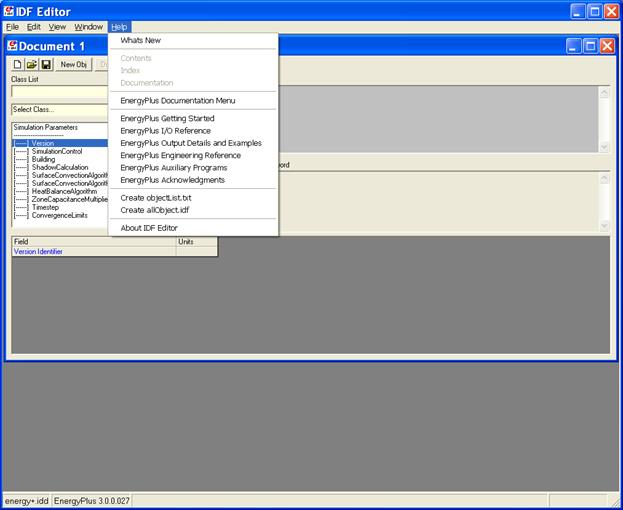
\includegraphics[width=0.9\textwidth, height=0.9\textheight, keepaspectratio=true]{media/image002.jpg}
\caption{Using IDFEditor to find the latest groups and objects for the Energy+.idd \protect \label{fig:using-idfeditor-to-find-the-latest-groups}}
\end{figure}

The produced list will look something like:

Simulation Parameters

\begin{center}\rule{0.5\linewidth}{0.4pt}\end{center}

{[}------{]}~ Version

{[}------{]}~ SimulationControl

{[}------{]}~ Building

{[}------{]}~ ShadowCalculation

{[}------{]}~ SurfaceConvectionAlgorithm:Inside

{[}------{]}~ SurfaceConvectionAlgorithm:Outside

{[}------{]}~ HeatBalanceAlgorithm

{[}------{]}~ ZoneCapacitanceMultiplier

{[}------{]}~ Timestep

{[}------{]}~ ConvergenceLimits

Location - Climate - Weather File Access

\begin{center}\rule{0.5\linewidth}{0.4pt}\end{center}

{[}------{]}~ Site:Location

{[}------{]}~ SizingPeriod:DesignDay

{[}------{]}~ SizingPeriod:WeatherFileDays

{[}------{]}~ SizingPeriod:WeatherFileConditionType

{[}------{]}~ RunPeriod

{[}------{]}~ RunPeriodControl:SpecialDays

{[}------{]}~ RunPeriodControl:DaylightSavingTime

``Simulation Parameters'' and ``Location -- Climate -- Weather File Access'' are groups. Version, Building, etc are objects.
